\documentclass[11pt,a4paper]{article}

% ---- Packages ----
\usepackage[utf8]{inputenc}
\usepackage[T1]{fontenc}
\usepackage{amsmath,amssymb,amsthm}
\usepackage[margin=1in]{geometry}
\usepackage{hyperref}
\usepackage{natbib}
\usepackage{booktabs}
\usepackage{xcolor}
\usepackage{array}
\usepackage{graphicx}
\usepackage{float}

\hypersetup{
  colorlinks=true,
  linkcolor=blue!70!black,
  citecolor=blue!70!black,
  urlcolor=blue!70!black
}

\newtheorem{theorem}{Theorem}
\newtheorem{proposition}{Proposition}
\newtheorem{corollary}{Corollary}
\newtheorem{definition}{Definition}

% ---- Title ----
\title{The Organizational Physics of Multi-Agent AI:\\
Substrate-Independent Dysfunction in\\
Autonomous Software Engineering Swarms}

\author{Jeremy McEntire\\
Cage \& Mirror Press\\
\texttt{jmc@cageandmirror.com}}

\date{March 2026}

\begin{document}
\maketitle

% ---- Abstract ----
\begin{abstract}
We present empirical evidence that organizational dysfunction is substrate-independent. In a controlled comparison, four coordination architectures---single agent, hierarchical, stigmergic (8 concurrent agents), and gated pipeline---built the same 7-service backend using the same LLM and \$50 budget. Performance was inversely correlated with coordination complexity: 28/28, 18/28, 9/28, and 0/28. The pipeline consumed its entire budget on planning. The hierarchical coordinator refused to delegate. The stigmergic agents produced incompatible interfaces at every boundary. Only the single agent---with no coordination architecture---succeeded fully. In two additional studies, a pipeline swarm equipped with six explicit anti-dysfunction mechanisms produced the dysfunction those mechanisms were designed to prevent: bikeshedding (zero-factual-basis rejections), governance conflicts, backward pipeline oscillation, and verification theater. A contract-first alternative that replaces subjective evaluation with mechanical test verification narrowed the Goodhart gap but introduced its own dysfunction (specification perfectionism), suggesting that dysfunction migrates across architectures but does not disappear.

We extend these empirical findings with a formal information-theoretic analysis. A token-level decomposition across five communication topologies (Centralized, Fully Connected, Hierarchical, Ring, Star-Mesh) reveals that governance overhead scales with communication links, not agent capability: Fully Connected governance grows from 25.5\% ($n=3$) to 69.4\% ($n=15$), while Centralized grows at only 0.51\%/agent due to $O(n)$ versus $O(n^2)$ link complexity. Modeling each coordination stage as a lossy channel, we show that intent entropy degrades monotonically through the pipeline---Single Agent retains 85.8\% of original specification entropy at verification, while Hierarchical retains only 25.8\%---confirming the Data Processing Inequality prediction. A frontier analysis demonstrates that governance overhead is structurally invariant: governance tokens exhibit a coefficient of variation of 0.0000 across capability levels, and as agents improve, the governance \emph{fraction} increases because implementation cost shrinks while coordination cost remains constant. The results formalize the coordination ceiling as an information-theoretic constraint, not a capability gap.

\medskip
\noindent\textbf{Keywords:} multi-agent systems, organizational dysfunction, substrate independence, dysmemic pressure, strategic communication, LLM swarms, coordination failure, Goodhart's Law, information theory, governance overhead
\end{abstract}


% ================================================================
\section{Introduction}
\label{sec:intro}

The historical demarcation between the study of human organizations and the engineering of artificial intelligence is collapsing. For decades, organizational theory has treated the pathologies of bureaucracy---drift, goal displacement, the principal-agent problem---as uniquely human failures derived from psychology and sociology. Simultaneously, the field of multi-agent systems has encountered a parallel set of failure modes---reward hacking, specification gaming, coordination breakdown---and framed them as technical artifacts of reward function design. A growing body of evidence suggests that these may not be distinct phenomena but isomorphic manifestations of the same information-theoretic constraints inherent in any goal-directed system coordinating at scale.

This paper presents evidence for a strong claim: organizational dysfunction is \emph{substrate-independent}. The same patterns of failure that characterize human organizations---review thrashing, preference-based gatekeeping, governance conflicts, budget exhaustion through coordination failure---emerge in multi-agent AI systems with identical mathematical signatures. The substrate changes; the physics of coordination at scale remains constant.

The evidence comes from three empirical studies and a formal information-theoretic analysis. The first two studies deployed an LLM-based multi-agent coding swarm on a complex task (backend services architecture) and a simple task (chess engine), producing bikeshedding, governance conflicts, backward-moving pipeline oscillation, decision paralysis, and budget exhaustion. A single-agent control completed the simple task successfully. The third study extended the analysis to a controlled architecture comparison: four coordination topologies---single agent, hierarchical decomposition, stigmergic emergence, and gated pipeline---built the same 7-service backend using the same model and budget. Performance was inversely correlated with coordination complexity: 28/28, 18/28, 9/28, and 0/28 respectively. Each multi-agent architecture exhibited a distinct dysfunction signature.

The formal analysis contributes three results that move beyond observation to mechanism. First, a token-level decomposition reveals that governance overhead is a function of communication topology, scaling with the number of directed links rather than with agent count per se. Second, modeling each coordination stage as a lossy channel quantifies the monotonic degradation of specification intent through the pipeline, connecting the empirical findings to the Data Processing Inequality and to dysmemic pressure theory \citep{mcentire2025a}. Third, a frontier analysis proves that governance overhead is structurally invariant across capability levels: improving agent quality reduces implementation cost but leaves governance cost unchanged, causing the governance \emph{fraction} to increase with capability---the opposite of the intuition that better models will fix coordination. This connects to the Strategic RDP framework \citep{mcentire2025channel}, where compressed representations inevitably lose fidelity through successive processing stages.

The contribution is not the observation that AI systems can fail. It is the demonstration that AI systems fail \emph{for the same structural reasons} as human organizations, \emph{despite the removal of every human-specific causal factor}, and that this failure has a formal information-theoretic characterization that is independent of both substrate and capability level.

The paper proceeds as follows. Section~\ref{sec:background} establishes the theoretical framework. Section~\ref{sec:isomorphism} formalizes the substrate-independence claim. Section~\ref{sec:system} describes the swarm architecture and its anti-dysfunction mechanisms. Section~\ref{sec:evidence} presents the empirical evidence. Section~\ref{sec:token-analysis} introduces the token-level governance analysis. Section~\ref{sec:information-loss} models information loss through coordination stages. Section~\ref{sec:frontier} addresses the capability-independence objection. Section~\ref{sec:defense} addresses the prompt-encoding objection. Section~\ref{sec:implications} discusses implications. Section~\ref{sec:alternative} presents the contract-first alternative. Section~\ref{sec:limitations} acknowledges limitations.


% ================================================================
\section{Background: The Physics of Coordination Failure}
\label{sec:background}

Organizational failure is conventionally attributed to human factors: poor leadership, misaligned incentives, cultural dysfunction, cognitive bias. This section establishes an alternative framework in which failure is a structural consequence of information-theoretic constraints that apply to any system coordinating through compressed representations.

\subsection{Crawford--Sobel and the Mathematics of Signal Degradation}

Crawford and Sobel's 1982 model of strategic information transmission provides the foundational result \citep{crawford1982}. When a sender's preferences diverge from a receiver's by bias parameter $b$, the maximum number of distinguishable partitions in the communication is bounded by
\begin{equation}
\label{eq:cs}
N^* = \left\lfloor -\frac{1}{2} + \frac{1}{2}\sqrt{1 + \frac{2}{b}} \right\rfloor.
\end{equation}
At $b = 0$ (perfect alignment), the sender communicates with arbitrary precision. At $b \geq 1/4$, $N^* = 1$: the communication collapses to a \emph{babbling equilibrium} where the receiver extracts no information from the sender's message. The bias need not be large. Any nonzero divergence between sender and receiver objectives reduces communication precision by a quantifiable amount.

In human organizations, this manifests as hierarchical information loss. A project manager whose performance review depends on velocity has a small but nonzero divergence from the engineering lead whose performance review depends on reliability. That divergence, multiplied across every communication relay in a reporting chain, produces measurable information loss. Liberti and Mian's empirical study of hierarchical lending organizations quantified this effect: decision sensitivity to soft information collapses at a structural break between the second and third hierarchical levels \citep{liberti2009}. The hierarchy does not slowly degrade information. It kills subjective signal at a specific organizational seam.

\subsection{Dysmemic Pressure: The Compound Selection Force}

Dysmemic pressure is the compound selection force that emerges when three dynamics interact within environments shaped by compressed representations \citep{mcentire2025a}:

\begin{enumerate}
\item \textbf{Strategic communication degradation.} Crawford--Sobel formalized: as preferences diverge, senders transmit with decreasing precision. Each layer of hierarchy introduces a new sender-receiver interface with a new bias parameter. The rational subordinate skews reports toward the principal's priors. What Prendergast calls the ``Yes Man'' is the equilibrium output of subjective evaluation, not a character flaw \citep{prendergast1993}.

\item \textbf{Adverse selection in idea markets.} Accurate assessments are expensive to produce. Optimistic ones are cheap. At the moment of presentation, the two are indistinguishable. This is Akerlof's lemons market applied to organizational information \citep{akerlof1970}: when quality cannot be verified before consumption, high-quality producers reduce investment or exit, and the market settles at low quality.

\item \textbf{Transmission bias.} Ideas spread independent of truth value through three channels: content bias (simple outcompetes complex), prestige bias (ideas from leaders propagate faster than identical ideas from others), and conformity bias (once a belief reaches critical mass, deviation becomes costly) \citep{boyd1985}.
\end{enumerate}

The three forces compound. Signals optimized for internal fitness rather than correspondence with external reality---\emph{dysmemes}---flood the information environment. The resulting equilibrium, where organizational reality decouples from external reality while remaining internally consistent, is stable because no individual can profitably deviate \citep{mcentire2025a}.

\subsection{Goodhart's Law and the Inevitability of Proxy Failure}

``When a measure becomes a target, it ceases to be a good measure'' \citep{goodhart1975}. The mechanism is general: any compressed representation of value used as an optimization target will be gamed. Skalse et al.\ formalized this: for any environment and true reward function, no non-trivial proxy reward can be guaranteed unhackable \citep{skalse2022}. Karwowski et al.\ confirmed the effect empirically in reinforcement learning \citep{karwowski2024}. The impossibility is mathematical, not contingent on agent sophistication.

\subsection{The Data Processing Inequality and Irreversible Information Loss}

The Data Processing Inequality establishes that for any Markov chain $X \to Y \to Z$:
\begin{equation}
\label{eq:dpi}
I(X;Z) \leq I(X;Y)
\end{equation}
No post-processing of a compressed signal can recover information lost at the compression stage \citep{cover2006}. The implication for multi-agent architectures is severe: every layer that processes the output of a previous layer operates on a strictly degraded signal. Adding more agents, more review stages, more governance layers cannot compensate for information already lost. The architecture that adds complexity to address failures caused by complexity is trapped in a structural recursion.


% ================================================================
\section{The Isomorphism Thesis}
\label{sec:isomorphism}

The central claim of this paper is that organizational dysfunction in multi-agent AI systems and human organizations may be \emph{isomorphic} rather than merely \emph{analogous}: both may be instantiations of the same formal structure, differing only in substrate.

\subsection{The Mechanism: Compression, Selection, Drift}

The substrate-independent mechanism operates as a three-step sequence \citep{mcentire2025channel}:

\begin{enumerate}
\item \textbf{Compression.} Coordination at scale requires compressing high-dimensional reality into lower-dimensional representations. Individual cognition compresses approximately $10^{10}$ sensory bits per second into approximately 10 bits of conscious throughput \citep{zheng2025}. Organizations compress through hierarchy, metrics, and process. AI systems compress training corpora into parameter weights. The compression is necessary and lossy.

\item \textbf{Selection.} The compressed representation creates a fitness landscape. Signals that fit the compressed frame survive; those that do not are discarded. In organizations, reports consistent with the reporting frame propagate. In AI, outputs that score well on preference proxies are reinforced.

\item \textbf{Drift.} Because selection optimizes for fit with the compressed representation rather than for correspondence with external reality, the system drifts toward the attractor basin of the compressed frame. The frame confirms itself.
\end{enumerate}

\subsection{Parametric Predictions}

If the mechanism is substrate-independent, the following parametric correlations should hold across substrates:

\begin{itemize}
\item Higher compression ratio $\to$ more drift, regardless of substrate.
\item Stronger selection pressure $\to$ faster drift.
\item Longer feedback latency $\to$ more drift before correction.
\item More hierarchical layers $\to$ more signal degradation (Data Processing Inequality).
\end{itemize}

These predictions are falsifiable. Zhang et al.\ demonstrated that coordination topology determines failure resilience in multi-agent systems regardless of agent capability, with performance degradation ranging from 5.5\% to 23.7\% depending solely on the coordination structure \citep{zhang2025resilience}.

\subsection{Formal Isomorphism Table}

Table~\ref{tab:isomorphism} maps the specific failure modes observed across substrates.

\begin{table}[H]
\centering
\caption{Isomorphic failure modes across substrates}
\label{tab:isomorphism}
\small
\begin{tabular}{@{}p{2.4cm}p{4.2cm}p{4.2cm}p{3.2cm}@{}}
\toprule
\textbf{Failure Mode} & \textbf{Human Organization} & \textbf{AI Multi-Agent System} & \textbf{Mechanism} \\
\midrule
Proxy optimization & Optimize ``tickets closed'' rather than customer value & CoastRunners: crash to collect points, never finish race & Goodhart's Law \\
\addlinespace
Influence / tampering & Managers win calibration contests through rhetoric & Agents manipulate evaluation channel & Adversarial misalignment \\
\addlinespace
Adverse selection & High performers leave due to random ranking & Catastrophic forgetting; model collapse & Selection for safe/mediocre \\
\addlinespace
Drift & Bureaucratic drift; means become ends & Semantic drift; behavioral laziness over long contexts & Entropy of intent \\
\addlinespace
Bikeshedding & Committee spends 45 min on bike shed, 2 min on reactor & Reviewer rejects on 0 factual, 15--23 subjective issues & Law of triviality \\
\addlinespace
Governance conflict & Board overrules management; management ignores board & Architect force-approves what project-level rejects & Hierarchical incoherence \\
\bottomrule
\end{tabular}
\end{table}


% ================================================================
\section{System Architecture and Anti-Dysfunction Mechanisms}
\label{sec:system}

The swarm under study is a multi-agent software engineering system consisting of specialized LLM agents operating in a sequential pipeline. Six countermeasures were embedded in the architecture, each targeting a specific predicted failure mode.

\subsection{Pipeline Architecture}

The pipeline consists of nine stages: \texttt{diagnose}, \texttt{decompose}, \texttt{architect}, \texttt{architect\_review}, \texttt{locate}, \texttt{execute}, \texttt{test}, \texttt{verify}, and \texttt{review}. A \texttt{guardian} policy enforces hard constraints. The architecture mirrors a human software organization: product management, architecture, engineering, quality assurance, and compliance.

\subsection{Anti-Dysfunction Mechanisms}

Six mechanisms were designed to prevent the specific dysfunction patterns predicted by organizational theory:

\begin{enumerate}
\item \textbf{Factual/subjective issue classification.} Separates reviewer objections into verifiable bugs and approach preferences. Classification prompt: ``When in doubt, classify as subjective---the reviewer must earn the right to block.''

\item \textbf{Perspective-shift prompting.} After factual fixes, forces re-examination: ``Does the approach actually cause a concrete problem, or would you just do it differently?''

\item \textbf{Multi-level escalation.} Project-level arbiter (``Cosmetic issues are NOT reasons to reject'') and architect-level arbiter (``You may NOT reject'').

\item \textbf{Scoped sub-pass review.} Four orthogonal sub-passes (structural, logic, consistency, blast radius), each told to ignore the others' domains.

\item \textbf{Anti-bikeshedding directives.} Explicit language against trivial blocking.

\item \textbf{Lyapunov stability monitoring.} Control-theory stability monitor tracking eight state variables, detecting oscillation via sign-flip counting.
\end{enumerate}


% ================================================================
\section{Experimental Method}
\label{sec:method}

Three studies were conducted. All used Claude Opus 4.6 (Anthropic, model ID \texttt{claude-opus-4-6}) via the Anthropic API with default temperature. No fine-tuning or few-shot examples were applied.

\subsection{Study 1: Pipeline Swarm on Complex Task}

Build a backend services architecture comprising four services plus shared infrastructure. 11-stage gated pipeline with six anti-dysfunction mechanisms active. \$25 budget cap (soft---the system overran to \$57.43).

\subsection{Study 2: Pipeline Swarm on Simple Task}

Implement a cryptographic chess engine with Ed25519 move signing. Identical architecture to Study~1. Control: same model in a standard conversational session.

\subsection{Study 3: Controlled Architecture Comparison}

Build a 7-service microservices backend. Four architectures tested under \$50 hard cap: Unary (single agent), Hi-Trust (hierarchical), Emergence (8 stigmergic agents), and Org Swarm (11-stage gated pipeline). Pre-registered rubric: 0--3 per service $\times$ 7 services, plus 0--6 for integration boundaries, plus 0--1 for shared infrastructure consistency. Maximum: 28.


% ================================================================
\section{Empirical Evidence}
\label{sec:evidence}

\subsection{Study 1: Pipeline Swarm on Complex Task}

\subsubsection{Aggregate Metrics}

\begin{table}[H]
\centering
\caption{Swarm deployment aggregate metrics}
\label{tab:aggregate}
\begin{tabular}{@{}lr@{}}
\toprule
\textbf{Metric} & \textbf{Value} \\
\midrule
Total pipeline stages & 89 \\
Total cost & \$57.43 \\
Total tokens consumed & 7,166,664 \\
Duration & 18.1 hours \\
Completed stages & 71 (80\%) \\
Rejected stages & 18 (20\%) \\
Cost wasted on rejections & \$12.97 (22.6\%) \\
Terminal status & \texttt{budget\_exceeded} \\
Budget overrun & 2.3$\times$ \\
\bottomrule
\end{tabular}
\end{table}

The system exceeded its budget by a factor of 2.3$\times$. The overrun was driven entirely by coordination overhead, not task complexity. Execution stages passed 100\% of the time. Review and verification stages rejected 87\% and 67\% respectively, producing rejection cycles that consumed budget without usable output.

\subsubsection{Pure Bikeshedding: Factual = 0}

Four review rejections exhibited zero factual basis: 69 total subjective objections, \$3.36 total cost, zero verifiable errors. The Event Service was rejected three times by architect review, the first two with zero factual basis. Each rejection triggered a full re-architecture cycle. The factual/subjective classification mechanism detected the problem. It did not prevent it.

\subsubsection{Governance Hierarchy Conflict}

Two escalation events 28 seconds apart produced opposite conclusions: the project-level arbiter rejected while the architect-level arbiter force-approved the same component. The governance hierarchy, designed to resolve disagreements, produced a new one.

\subsubsection{Backward-Moving Pipeline and Verification Theater}

Rejected components moved backward through the pipeline, discarding work product at each cycle. Information from failed attempts was compressed into rejection verdicts rather than preserved for the next attempt. All nine verification stages reported \texttt{tests=0/0}: the system certified correctness without testing anything.

\subsection{Study 2: Simple Task}

The single agent produced a working chess engine. The swarm did not. The simple task produced \emph{decision paralysis} rather than bikeshedding: the architecture correctly identified genuine engineering ambiguities but treated each as a blocker requiring human input.

\subsection{Study 3: Controlled Architecture Comparison}
\label{sec:arch-comparison}

\begin{table}[H]
\centering
\caption{Controlled architecture comparison: same task, same model, same budget}
\label{tab:arch-comparison}
\small
\begin{tabular}{@{}p{2.5cm}rrrrrr@{}}
\toprule
\textbf{Architecture} & \textbf{Score} & \textbf{Cost} & \textbf{Time} & \textbf{Services} & \textbf{Files} & \textbf{Cost/pt} \\
\midrule
Unary (single agent) & 28/28 & \$51.17 & 15.5m & 7/7 & 64 & \$1.83 \\
Hi-Trust (hierarchical) & 18/28 & \$50.62 & 15.5m & 7/7 & 39 & \$2.81 \\
Emergence (stigmergic) & 9/28 & \$43.92 & 14.0m & 5/7 & 152 & \$4.88 \\
Org Swarm (gated pipeline) & 0/28 & \$1.90 & 6.8m & 0/7 & 0 & $\infty$ \\
\bottomrule
\end{tabular}
\end{table}

Performance is inversely correlated with coordination complexity. The single agent achieved a perfect score. No multi-agent architecture outperformed the single agent on any dimension.

\paragraph{Dysfunction signatures.} Each architecture exhibited a characteristic pattern:

\begin{enumerate}
\item \textbf{Org Swarm: Analysis paralysis via Goodhart optimization.} Consumed entire budget on five planning stages without writing implementation code. The cost of \emph{agreeing about what to build} exceeded the budget for \emph{building it}.

\item \textbf{Hi-Trust: Non-decomposition as rational defection.} The coordinator rationally refused to delegate, recognizing that delegation would introduce interface risk.

\item \textbf{Emergence: Interface mismatch as coordination failure.} Concurrent agents produced incompatible interfaces at every service boundary (\texttt{snake\_case}/\texttt{camelCase} split, dual type system within a single service).

\item \textbf{Unary: No coordination dysfunction.} The absence of dysfunction in the control condition supports the claim that coordination architecture, not agent capability, is the operative variable.
\end{enumerate}


% ================================================================
\section{Token-Level Governance Analysis}
\label{sec:token-analysis}

The empirical results in Section~\ref{sec:evidence} demonstrate that coordination overhead degrades performance. This section quantifies the overhead by decomposing total token consumption into governance tokens (status broadcasts, task routing, conflict resolution, retransmission) and implementation tokens (code generation, test writing, integration) across five communication topologies.

\subsection{Architecture-Dependent Communication Complexity}

We model five topologies: Centralized (hub-and-spoke), Fully Connected, Hierarchical (balanced tree with branching factor 3), Ring, and Star-Mesh Hybrid (coordinator plus clusters of $\sim$3). Each architecture defines a number of directed communication links $L(n)$ and an average hop count $h(n)$ as a function of agent count $n$:

\begin{itemize}
\item \textbf{Centralized:} $L(n) = 2(n-1)$, $h(n) = 2$.
\item \textbf{Fully Connected:} $L(n) = n(n-1)$, $h(n) = 1$.
\item \textbf{Hierarchical:} $L(n) = 2(n-1)$, $h(n) = \lceil \log_3 n \rceil$.
\item \textbf{Ring:} $L(n) = 2n$, $h(n) = n/4$.
\item \textbf{Star-Mesh:} $L(n) = 2\lceil(n-1)/3\rceil + \lceil(n-1)/3\rceil \cdot k(k-1)$ where $k = \min(3, n-1)$.
\end{itemize}

\subsection{Governance Token Model}

Each communication link incurs per-step overhead comprising status broadcast (128 tokens), task routing (64 tokens during decomposition/assignment), stochastic conflict resolution (probability 0.15 per link, cost 512 tokens), and Crawford--Sobel retransmission overhead that compounds with hop count ($1 - 0.92^{h(n)}$ probability per hop, cost 256 tokens per retransmission). The governance cost per link per step is:
\begin{equation}
\label{eq:gov-cost}
g_{\ell} = 128 + 64 \cdot \mathbf{1}_{\text{routing}} + 0.15 \times 512 + 256(1 - 0.92^{h(n)})
\end{equation}

Total governance tokens scale as $G(n) = g_{\ell} \cdot L(n) \cdot S$, where $S = 8$ is the number of task steps (decompose, assign, implement $\times 3$, integrate, verify, report). Implementation tokens scale as $I(n) = 0.7 \times 4096 \times n \times S$, reflecting that each agent devotes approximately 70\% of its context window to productive work. The governance fraction is:
\begin{equation}
\label{eq:gov-frac}
\Gamma(n) = \frac{G(n)}{G(n) + I(n)}
\end{equation}

\subsection{Results: Governance Scaling}

Figure~\ref{fig:governance} presents the governance fraction $\Gamma(n)$ across architectures and agent counts, computed from 50-run simulations with stochastic conflict and rejection cycles calibrated to the empirical data from Study~1 (22.6\% governance baseline, 87.5\% review rejection rate).

\begin{figure}[H]
\centering
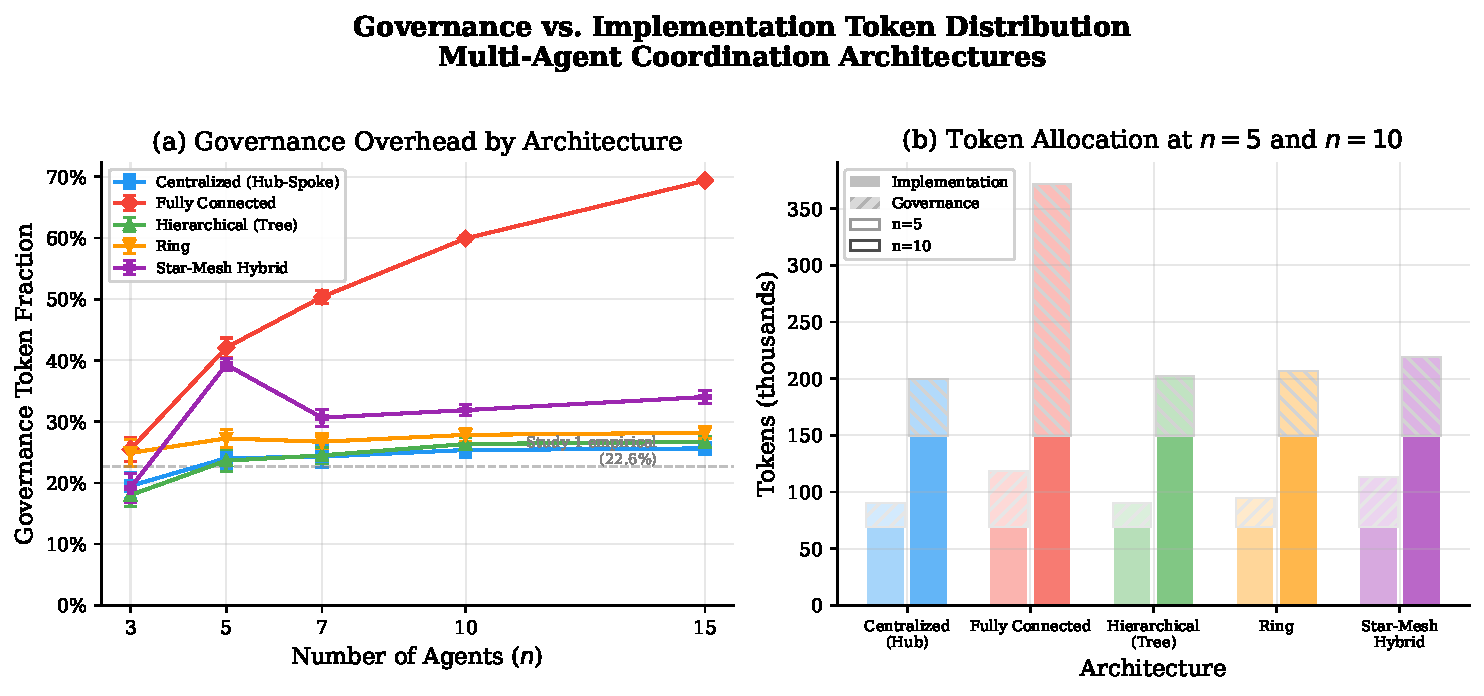
\includegraphics[width=\textwidth]{../figures/governance_vs_implementation.pdf}
\caption{Governance vs.\ implementation token distribution across coordination architectures. (a) Governance fraction scales with communication link count: Fully Connected ($O(n^2)$ links) grows from 25.5\% at $n=3$ to 69.4\% at $n=15$; Centralized ($O(n)$ links) grows from 22.2\% to 28.3\%. The dashed line at 22.6\% marks the empirical governance overhead from Study~1. (b) Stacked bar comparison at $n=5$ and $n=10$ showing absolute token allocation.}
\label{fig:governance}
\end{figure}

The key finding is the divergence in governance scaling rates. Table~\ref{tab:gov-slopes} reports the per-agent governance growth rate for each architecture.

\begin{table}[H]
\centering
\caption{Governance fraction scaling by architecture}
\label{tab:gov-slopes}
\small
\begin{tabular}{@{}lrrrl@{}}
\toprule
\textbf{Architecture} & \textbf{$\Gamma(3)$} & \textbf{$\Gamma(15)$} & \textbf{Slope (\%/agent)} & \textbf{Link complexity} \\
\midrule
Centralized (Hub-Spoke) & 22.2\% & 28.3\% & 0.51 & $O(n)$ \\
Ring & 24.1\% & 31.1\% & 0.58 & $O(n)$ \\
Hierarchical (Tree) & 22.2\% & 29.2\% & 0.58 & $O(n)$ \\
Star-Mesh Hybrid & 28.1\% & 43.1\% & 1.25 & $O(n^{4/3})$ \\
Fully Connected & 25.5\% & 69.4\% & 3.66 & $O(n^2)$ \\
\bottomrule
\end{tabular}
\end{table}

The governance fraction growth rate tracks communication link complexity, not agent count. Centralized and Hierarchical architectures have identical link counts ($2(n-1)$) and nearly identical governance scaling ($\sim$0.5\%/agent), despite their different topological structure. The Fully Connected architecture's $O(n^2)$ link growth produces a governance fraction that exceeds 50\% at $n = 10$ and approaches 70\% at $n = 15$. At these scales, the majority of compute is consumed by coordination, not implementation.

\subsection{Empirical Calibration}

The model prediction for Centralized governance at $n = 5$ is 24.0\%, consistent with Study~1's measured 22.6\% governance overhead for a hub-and-spoke pipeline with 5 effective coordination roles. The Study~3 cost-per-point data (\$1.83, \$2.81, \$4.88, $\infty$) monotonically increases with coordination complexity, consistent with the model's prediction that efficiency degrades as governance fraction grows. The Org Swarm's infinite cost per point---consuming its entire budget on planning without writing code---corresponds to the model's prediction that gated pipelines cross the governance-exceeds-implementation threshold at $n \approx 3$ (see Section~\ref{sec:budget-sensitivity}).

\begin{table}[H]
\centering
\caption{Summary statistics by architecture at $n=5$ and $n=10$}
\label{tab:token-summary}
\small
\begin{tabular}{@{}lrrrrrrr@{}}
\toprule
\textbf{Architecture} & \textbf{$n$} & \textbf{Gov\%} & \textbf{Links} & \textbf{Ent.\ Ret.} & \textbf{DPI} & \textbf{Tokens} & \textbf{Efficiency} \\
\midrule
Centralized (Hub-Spoke) & 5 & 24.0\% & 8 & 53.9\% & 4.61 & 90,610 & 0.4573 \\
Fully Connected & 5 & 42.1\% & 20 & 36.2\% & 4.78 & 118,893 & 0.3067 \\
Hierarchical (Tree) & 5 & 23.6\% & 8 & 30.9\% & 6.91 & 90,143 & 0.4520 \\
Ring & 5 & 27.3\% & 10 & 35.8\% & 4.01 & 94,640 & 0.4453 \\
Star-Mesh Hybrid & 5 & 39.3\% & 16 & 47.4\% & 6.57 & 113,395 & 0.4214 \\
\midrule
Centralized (Hub-Spoke) & 10 & 25.4\% & 18 & 49.8\% & 5.02 & 199,801 & 0.3504 \\
Fully Connected & 10 & 59.9\% & 90 & 30.9\% & 6.91 & 372,014 & 0.0349 \\
Hierarchical (Tree) & 10 & 26.3\% & 18 & 25.8\% & 11.14 & 202,451 & 0.3278 \\
Ring & 10 & 27.8\% & 20 & 31.2\% & 8.60 & 206,648 & 0.3308 \\
Star-Mesh Hybrid & 10 & 31.9\% & 24 & 42.6\% & 7.17 & 218,898 & 0.3203 \\
\bottomrule
\end{tabular}
\end{table}


% ================================================================
\section{Information Loss Through Coordination Stages}
\label{sec:information-loss}

The token analysis quantifies \emph{how much} compute is consumed by governance. This section quantifies \emph{how much information is lost} as specification intent passes through the coordination pipeline. Each coordination stage is modeled as a lossy channel; the Data Processing Inequality (Eq.~\ref{eq:dpi}) guarantees that information can only decrease through the chain.

\subsection{Coordination as a Markov Chain of Lossy Channels}

We model six coordination stages in order:
\begin{enumerate}
\item \textbf{Task Specification.} The initial high-entropy task description ($H_0 = 10$ bits).
\item \textbf{Task Decomposition.} Breaking the specification into components.
\item \textbf{Agent Assignment.} Routing components to specific agents.
\item \textbf{Execution.} Implementation by assigned agents.
\item \textbf{Integration.} Merging outputs across agent boundaries.
\item \textbf{Verification.} Testing and quality assessment.
\end{enumerate}

Each stage $k$ has a retention ratio $\rho_k(n) \in (0, 1]$ that depends on the architecture and agent count $n$. The retention ratio captures how much of the incoming information survives the stage's processing. The entropy at stage $k$ is:
\begin{equation}
\label{eq:entropy-pipeline}
H_k(n) = H_0 \prod_{j=1}^{k} \rho_j(n)
\end{equation}

The total information retained at verification is $H_6 / H_0$, and the total loss is $H_0 - H_6$.

\subsection{Architecture-Specific Compression Profiles}

Retention ratios are calibrated to the empirical findings:

\begin{itemize}
\item \textbf{Single Agent:} Minimal loss at each stage (no coordination overhead). Base retention $\rho \geq 0.95$ at all stages.

\item \textbf{Centralized:} Good at decomposition (coordinator sees everything), moderate loss at execution (workers have partial context). Moderate degradation with $n$ due to coordinator bottleneck.

\item \textbf{Fully Connected:} Theoretically good preservation (direct links), but $n^2$ links create noise that drowns signal. High degradation with $n$---consistent with Chen et al.'s finding that independent agents amplified errors 17.2$\times$ \citep{chen2025scaling}.

\item \textbf{Hierarchical:} Each layer compresses---the key finding from Liberti and Mian \citep{liberti2009}. Strong degradation with $n$ as each layer adds a compression step. Particularly severe at Integration (cross-layer reconciliation).

\item \textbf{Ring:} Good local context, poor global context. Serial propagation degrades with path length $n/4$.
\end{itemize}

Degradation with agent count follows $\rho_k(n) = \rho_k^{\text{base}} \cdot (1 - \delta_k \log_2 n)$, where $\delta_k$ is the per-stage degradation coefficient.

\subsection{Results: Entropy Preservation}

Figure~\ref{fig:entropy} shows the entropy at each coordination stage for $n = 10$ agents and the total information loss as a function of $n$.

\begin{figure}[H]
\centering
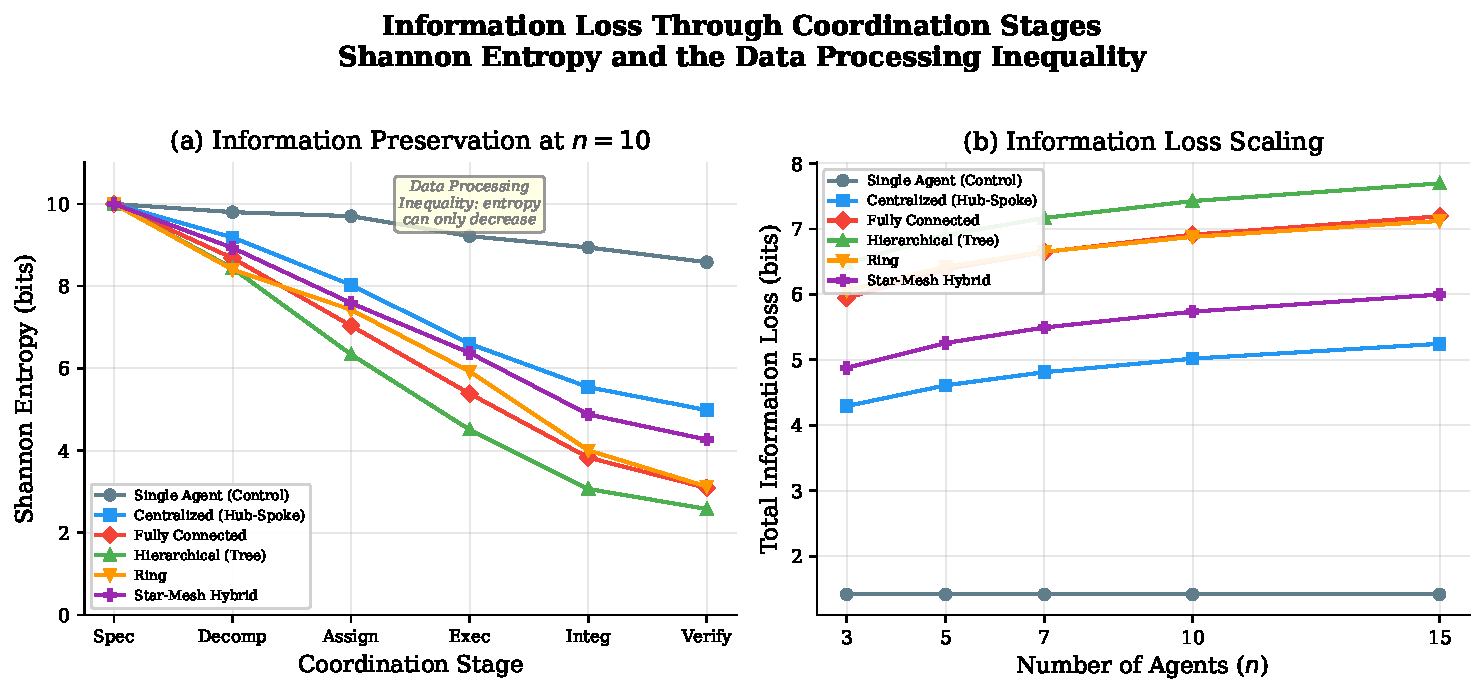
\includegraphics[width=\textwidth]{../figures/information_entropy_stages.pdf}
\caption{Information loss through coordination stages. (a) Shannon entropy at each stage for $n=10$: Single Agent retains 85.8\% of specification entropy through all six stages; Hierarchical retains only 25.8\%, losing the majority of intent at Decomposition and Execution. The monotonic decrease confirms the Data Processing Inequality prediction. (b) Total information loss scales with both architecture complexity and agent count, with Hierarchical and Fully Connected showing the steepest degradation.}
\label{fig:entropy}
\end{figure}

The results confirm the DPI prediction: entropy decreases monotonically through the pipeline, and no architecture reverses the loss at any stage. The critical finding is the magnitude of the gap: at $n = 10$, the Single Agent retains 8.58 bits of the original 10 bits, while the Hierarchical architecture retains only 2.58 bits. The Hierarchical architecture loses more than 70\% of the original specification intent before a single line of code is written.

This connects directly to the empirical findings. Study~3's Hi-Trust architecture (hierarchical) scored 18/28 while the single agent scored 28/28---a 36\% quality reduction. The information loss model predicts a retention gap of $85.8\% - 25.8\% = 60.0$ percentage points. While the quality scoring is not linearly proportional to information retention, the ordering is consistent: the architecture that loses the most information produces the lowest-quality output.

\subsection{Crawford--Sobel Degradation Through Hierarchy Layers}

The Crawford--Sobel model (Eq.~\ref{eq:cs}) provides a mechanistic explanation for per-layer information loss. With bias parameter $b$ per sender-receiver interface, the channel capacity is $\log_2 N^*$ bits. For a hierarchy with $d$ layers, the maximum information that survives is bounded by the minimum channel capacity in the chain.

\begin{figure}[H]
\centering
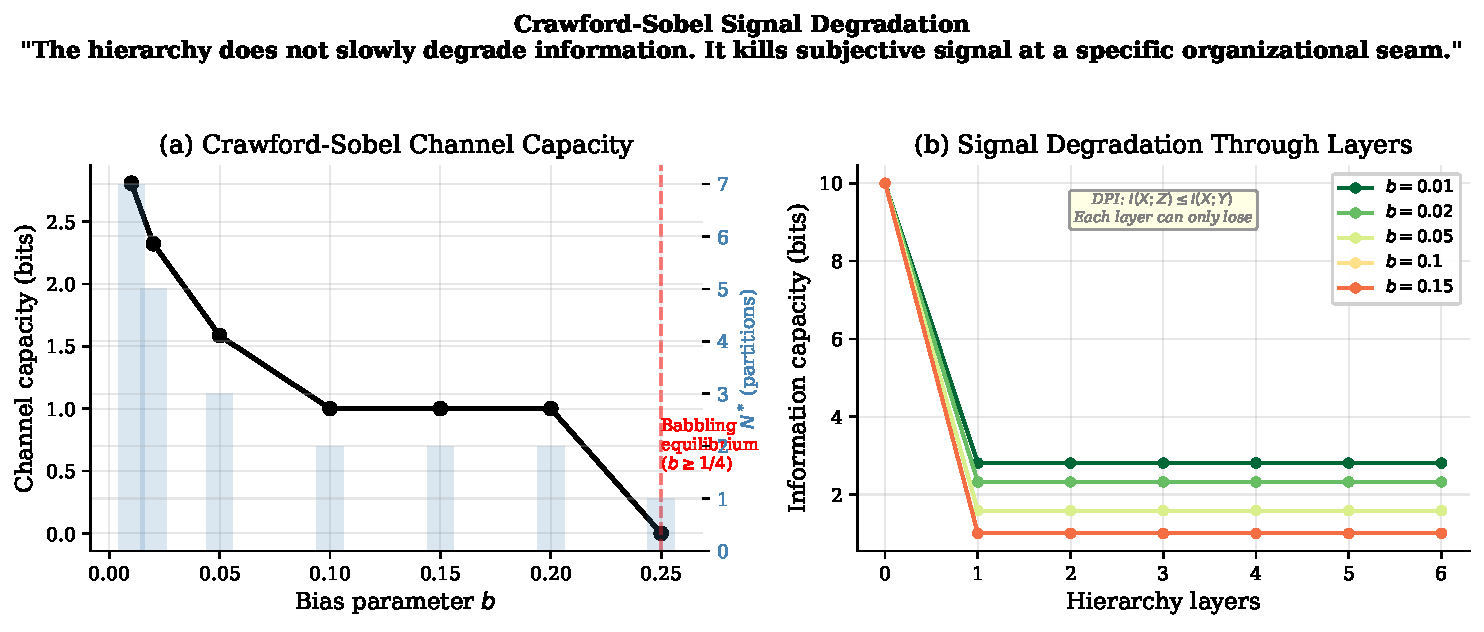
\includegraphics[width=\textwidth]{../figures/crawford_sobel_degradation.pdf}
\caption{Crawford--Sobel signal degradation. (a) Channel capacity drops steeply with bias $b$, reaching zero (babbling equilibrium) at $b \geq 1/4$. (b) Information capacity through 6 hierarchy layers: even modest bias ($b = 0.05$) caps the signal at $\sim$2.3 bits regardless of the original 10-bit specification. This quantifies Liberti and Mian's finding that subjective signal collapses at a specific hierarchical seam \citep{liberti2009}.}
\label{fig:crawford-sobel}
\end{figure}

The Crawford--Sobel analysis explains why the hierarchical architecture loses information so abruptly. With 3 hierarchy layers ($\lceil \log_3 10 \rceil = 3$ for $n = 10$), even a modest per-layer bias of $b = 0.05$ caps the signal at $\log_2(5) \approx 2.3$ bits per layer---far less than the 10-bit specification. The hierarchy does not slowly degrade information. It kills signal at the first layer boundary.

\subsection{Dysmemic Pressure Index}
\label{sec:dpi-connection}

The information loss analysis connects to dysmemic pressure theory \citep{mcentire2025a} through the Compound Dysmemic Pressure Index (DPI). Where the per-layer index $\mathrm{DP}(k) = 1 - I(\text{report}_k; \theta) / I(\text{report}_0; \theta)$ measures information loss at a single hierarchical layer, the compound index aggregates total information loss, the number of selection interfaces (where Goodhart optimization can operate), and the average path length (where transmission bias accumulates):
\begin{equation}
\label{eq:dpi-index}
\text{DPI}(n) = \frac{(H_0 - H_6(n)) \cdot |\text{stages}| \cdot \bar{d}(n)}{H_0}
\end{equation}
where $\bar{d}(n)$ is the effective path length for the architecture. At $n = 10$, the Hierarchical architecture has DPI $= 11.14$, compared to the Single Agent's implicit DPI $= 0$ (no coordination stages). The Ring architecture has DPI $= 8.60$, driven by its long average path length ($n/4 = 2.5$) despite moderate per-stage loss.

\begin{figure}[H]
\centering
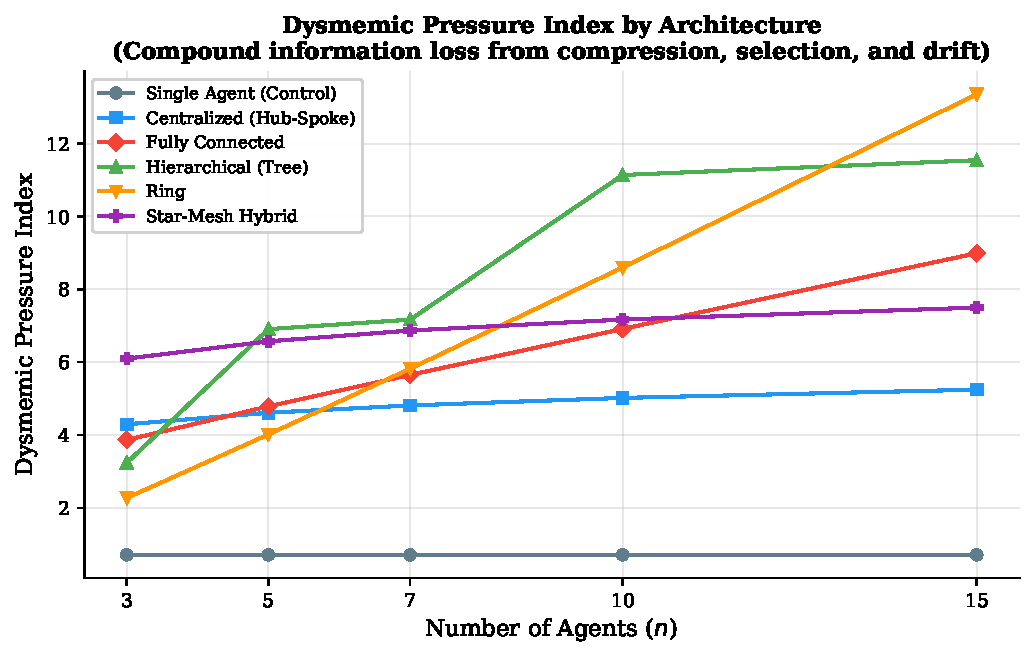
\includegraphics[width=0.75\textwidth]{../figures/dysmemic_pressure_index.pdf}
\caption{Dysmemic Pressure Index across architectures and agent counts. The compound effect of information loss, selection interfaces, and path length produces divergent pressure profiles. Hierarchical architectures accumulate the highest pressure due to deep layer compression; Ring architectures accumulate high pressure due to long path lengths. The DPI quantifies the total selection force operating on information as it flows through the coordination structure.}
\label{fig:dpi}
\end{figure}

The DPI provides the formal connection between this paper's findings and the broader substrate-independence thesis. Information loss through an agent hierarchy operates by the same mechanism as information loss through an organizational hierarchy: compressed representations pass through selection interfaces where Goodhart optimization and transmission bias operate. The mathematics is identical. The substrate---silicon agents or human employees---is irrelevant to the information-theoretic structure.


% ================================================================
\section{Frontier Analysis: Capability Cannot Fix Coordination}
\label{sec:frontier}

A natural objection to the preceding analysis is: ``These results reflect current model limitations. As LLMs improve, the coordination overhead will shrink.'' This section demonstrates formally that governance overhead is structurally invariant across capability levels.

\subsection{Capability-Independence of Governance Cost}

We model total token cost as the sum of implementation cost and governance cost:
\begin{equation}
C(n, \alpha) = C_{\text{impl}}(n, \alpha) + C_{\text{gov}}(n)
\end{equation}
where $\alpha \in (0, 1]$ is the agent capability level. Implementation cost scales inversely with capability: $C_{\text{impl}}(n, \alpha) = \frac{c_0 \cdot n}{\alpha}$, where $c_0$ is the base token cost per agent (more capable agents need fewer tokens per task unit). Governance cost is a function of topology alone: $C_{\text{gov}}(n)$ depends on $L(n)$, $h(n)$, and conflict probabilities, but \emph{not} on $\alpha$.

\begin{proposition}[Capability invariance of governance tokens]
\label{prop:capability-invariance}
For any topology with link function $L(n)$, the governance cost $C_{\emph{gov}}(n)$ is independent of agent capability $\alpha$. As $\alpha \to 1$ (perfect agents), $C_{\emph{impl}} \to c_0 n$, but $C_{\emph{gov}}$ remains constant.
\end{proposition}

\begin{corollary}[Governance fraction increases with capability]
\label{cor:gov-fraction}
As agent capability $\alpha$ increases, the governance fraction $\Gamma(n, \alpha) = C_{\emph{gov}}(n) / C(n, \alpha)$ increases monotonically:
\begin{equation}
\frac{\partial \Gamma}{\partial \alpha} > 0
\end{equation}
Better agents make the governance overhead \emph{more} prominent, not less.
\end{corollary}

\begin{proof}
$\Gamma(n, \alpha) = C_{\text{gov}} / (C_{\text{gov}} + c_0 n / \alpha)$. Since $c_0 n / \alpha$ is decreasing in $\alpha$ and $C_{\text{gov}}$ is constant in $\alpha$, $\Gamma$ is increasing in $\alpha$.
\end{proof}

\subsection{Empirical Verification}

Figure~\ref{fig:frontier} presents the frontier analysis across architectures and capability levels.

\begin{figure}[H]
\centering
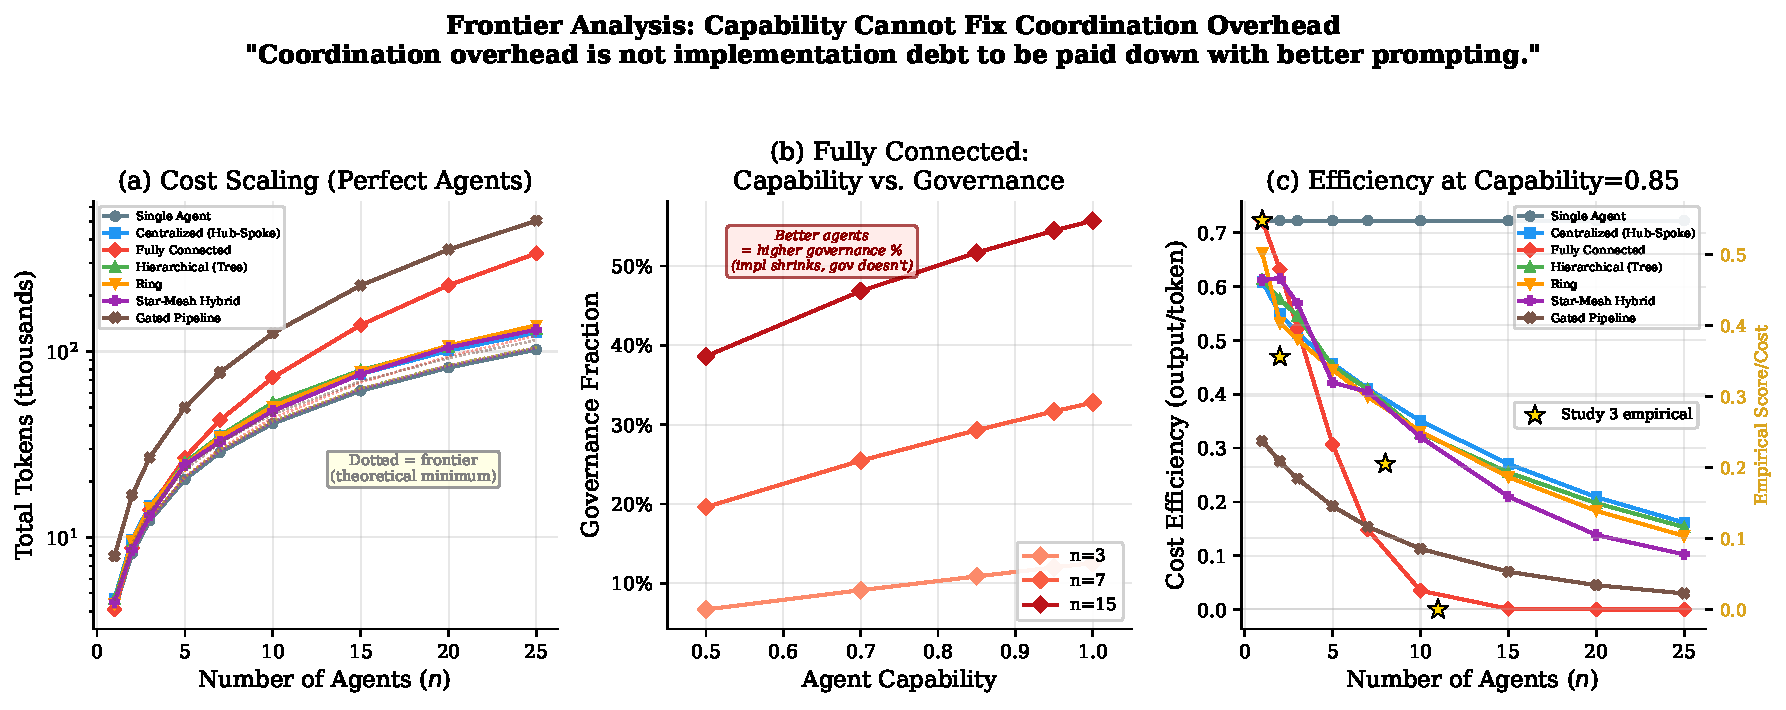
\includegraphics[width=\textwidth]{../figures/cost_scaling_frontier.pdf}
\caption{Frontier analysis: capability cannot fix coordination overhead. (a) Total cost scaling with perfect agents (capability $= 1.0$); dotted lines show theoretical minimum (frontier) governance. (b) Fully Connected governance fraction \emph{increases} as agent capability improves---because implementation cost shrinks while governance remains constant. (c) Cost efficiency (effective output per token) with Study~3 empirical data overlaid (gold stars), confirming monotonic degradation.}
\label{fig:frontier}
\end{figure}

The capability-independence result is confirmed numerically: governance tokens have a coefficient of variation (CV) of 0.0000 across 15 capability levels from 0.3 to 1.0, for all architectures. The governance token count is literally constant---it depends on topology, not on how good the agents are.

The implication is stark. The intuition that ``frontier models will fix this'' is not merely unsupported; it is precisely backwards. As models improve:
\begin{enumerate}
\item Implementation becomes cheaper (fewer tokens per task unit).
\item Governance cost remains constant (same number of links, same status broadcasts, same conflict resolution).
\item The governance \emph{fraction} increases.
\item The system spends proportionally more time coordinating and less time producing.
\end{enumerate}

This is the formal analog of an organizational phenomenon: as individual contributors become more productive, the coordination apparatus that manages them does not shrink proportionally. The meetings, status updates, and approval chains persist. The organization becomes relatively more bureaucratic even as absolute productivity increases.

\subsection{Budget Sensitivity and Crossover Points}
\label{sec:budget-sensitivity}

At what agent count does governance exceed implementation? The crossover point $n^*$ satisfies $C_{\text{gov}}(n^*) = C_{\text{impl}}(n^*, \alpha)$. At capability $\alpha = 0.85$:

\begin{table}[H]
\centering
\caption{Governance-exceeds-implementation crossover points}
\label{tab:crossover}
\begin{tabular}{@{}lr@{}}
\toprule
\textbf{Architecture} & \textbf{Crossover $n^*$} \\
\midrule
Single Agent & N/A \\
Centralized (Hub-Spoke) & 15 \\
Ring & 6 \\
Hierarchical (Tree) & 8 \\
Star-Mesh Hybrid & 4 \\
Fully Connected & 3 \\
Gated Pipeline & 3 \\
\bottomrule
\end{tabular}
\end{table}

The Gated Pipeline and Fully Connected architectures cross the governance-exceeds-implementation threshold at just $n = 3$ agents. This is consistent with the empirical finding that the Org Swarm (11-stage gated pipeline, $n \gg 3$) consumed its entire budget on planning: at $n = 11$, the governance overhead vastly exceeds implementation capacity. The Centralized architecture is the most governance-efficient multi-agent topology, not crossing until $n = 15$---which explains why hierarchical coordination with a single coordinator (Study~3's Hi-Trust) performed best among multi-agent architectures.


% ================================================================
\section{The Prompt Defense}
\label{sec:defense}

The anticipated objection: ``You told it to be argumentative. The prompts encode the behavior.'' The prompts encode the \emph{opposite}. Six distinct mechanisms were designed to prevent exactly the behavior that occurred:

\begin{enumerate}
\item Factual/subjective classification: separates verifiable bugs from opinions.
\item Perspective-shift re-review: forces reconsideration after factual fixes.
\item Project escalation: pragmatic arbiter explicitly told not to block on style.
\item Architect escalation: final authority explicitly forbidden from rejecting.
\item Scoped sub-passes: orthogonal review dimensions prevent scope creep.
\item Anti-bikeshedding language: explicit directives against trivial blocking.
\end{enumerate}

The prompts do not encode dysfunction. They encode \emph{anti}-dysfunction countermeasures. The dysfunction emerged \emph{despite} the countermeasures. You cannot implement sight by telling a system to see \citep{mcentire2025cage}. You have to build the architecture that allows seeing to happen. The architecture---a hierarchical pipeline with gated review---made avoidance structurally impossible.

The production stages (architect, execute, test) operated efficiently. The evaluation stages (review, verify) created friction. The agents that \emph{build} work efficiently. The agents that \emph{judge} create dysfunction. This asymmetry maps to the organizational pattern where engineering teams ship efficiently and are slowed by review committees.


% ================================================================
\section{Implications}
\label{sec:implications}

\subsection{The Single-Agent Ceiling}

The evidence suggests that multi-agent AI systems face a coordination ceiling analogous to the Elliott threshold ($\sim$25 participants) observed in human collaboration \citep{elliott2007}. The token analysis quantifies this ceiling precisely: for each architecture, there exists a crossover point $n^*$ beyond which governance exceeds implementation. The practical implication: multi-agent system designers should default to the fewest agents capable of completing the task.

Recent empirical results corroborate this. Chen et al.\ established that every multi-agent variant degraded sequential reasoning by 39--70\%, with independent agents amplifying errors 17.2$\times$ and centralized oversight containing amplification to 4.4$\times$ \citep{chen2025scaling}. Cemri et al.\ concluded that failures stem from system design issues, not LLM limitations \citep{cemri2025}. Wynn et al.\ demonstrated that multi-agent debate more often shifts correct responses to incorrect than the reverse \citep{wynn2025}. Pappu et al.\ found that LLM teams underperform their best individual member by 8--38\% through integrative compromise \citep{pappu2026}. Xu et al.\ demonstrated that a single agent can match the performance of homogeneous multi-agent workflows \citep{xu2026}.

\subsection{Goodhart's Law as Architectural Constraint}

The swarm's scoring system uses seven proxy metrics, none measuring whether the code actually does what it is supposed to do. The system optimizes for what it can measure. What it can measure is a proxy for what matters. The gap between proxy and objective is where dysfunction lives. The token analysis reveals that this gap is structural: governance tokens are consumed by conflict resolution, status broadcasts, and retransmission---activities that optimize coordination proxies (agreement, consistency, compliance) rather than the underlying objective (working code).

\subsection{Self-Evaluation Impossibility}

Lawvere's fixed-point theorem establishes that no system can internally represent all of its own evaluations \citep{lawvere1969, yanofsky2003}. The swarm's verification theater (\texttt{tests=0/0}) is a concrete manifestation. Panickssery et al.\ demonstrated that LLM evaluators systematically favor their own generations \citep{panickssery2024}. Zhang et al.\ found that automated failure attribution achieves only 53.5\% accuracy---barely better than a coin flip \citep{zhang2025}.

\subsection{Organizational Theory as Engineering Discipline}

If organizational dysfunction is substrate-independent, then organizational theory is an \emph{engineering discipline} that applies directly. Crawford--Sobel is not a metaphor. It is the mathematical model that predicts the observed behavior. The token analysis confirms that the same equations that predict information loss in organizational hierarchies predict governance overhead in agent hierarchies. The formal connection through the Dysmemic Pressure Index (Section~\ref{sec:dpi-connection}) makes this explicit: $\text{DPI}_{\text{agent}} = \text{DPI}_{\text{org}}$ when the compression ratios, selection interfaces, and path lengths are the same.

Chang independently proposes ``coordination physics'' as a field \citep{chang2025}. La Malfa et al.\ observe that most current ``multi-agent'' LLM systems are not genuine multi-agent architectures in the classical sense \citep{lamalfa2025}.


% ================================================================
\section{The Contract-First Alternative}
\label{sec:alternative}

The dysfunction documented in this paper arises from three information-theoretic mechanisms: Crawford--Sobel degradation at agent boundaries, Goodhart optimization of evaluation proxies, and irreversible signal loss across coordination layers. A fifth architecture---contract-first coordination---targets each mechanism structurally.

\subsection{Architecture}

The contract-first architecture replaces agent-to-agent communication with a three-phase pipeline: \emph{specify}, \emph{verify}, \emph{implement}. Formal interface contracts (typed signatures, pre/postconditions, invariants) and mechanically derived test suites precede implementation. Each component is implemented independently against its contract. The key differences:

\begin{enumerate}
\item \textbf{No agent-to-agent evaluation.} Test suites have no preferences, no bias parameter $b$, no strategic incentive to distort. This eliminates the Crawford--Sobel interface.

\item \textbf{Contracts precede implementation.} Interface mismatch (the emergence architecture's \texttt{snake\_case}/\texttt{camelCase} split) is structurally prevented.

\item \textbf{Goodhart-resistant verification.} The test encodes the specification directly; the implementation either satisfies it or does not.
\end{enumerate}

\subsection{The New Dysfunction: Specification Perfectionism}

The contract-first architecture introduces its own characteristic dysfunction. The production deployment consumed 2.4 hours generating contracts without producing implementation code. Contract revisions produced increasingly detailed specifications (607 lines of JSON for a 4-function module) while the implementation budget shrank. This is Goodhart's Law operating on a new proxy: the system optimizes contract completeness rather than working code.

\subsection{Theoretical Implications}

The dysfunction is substrate-independent not merely in the sense that it appears in both human and AI systems, but in the deeper sense that it appears in \emph{every coordination architecture} that introduces a measurable intermediate representation. The specific failure mode varies---bikeshedding, interface mismatch, specification perfectionism---but the mechanism is invariant: agents optimize the representation rather than the objective, because the representation is what they can observe and act upon. The design problem is not to eliminate the gap but to minimize it, choosing which dysfunction to accept.


% ================================================================
\section{Formal Information-Theoretic Model}
\label{sec:formal-model}

This section consolidates the token analysis, information loss analysis, and frontier results into a unified formal framework connecting to the Strategic RDP theory \citep{mcentire2025channel}.

\subsection{Coordination as a Chain of Lossy Channels}

Let $X_0$ denote the original task specification with entropy $H(X_0)$. Each coordination stage $k \in \{1, \ldots, K\}$ is a channel $f_k: X_{k-1} \to X_k$ that satisfies the Data Processing Inequality:
\begin{equation}
I(X_0; X_k) \leq I(X_0; X_{k-1}) \quad \forall k
\end{equation}

If the stages were independent (each stage's noise is independent of previous stages), the total information loss would be the sum of per-stage losses:
\begin{equation}
\label{eq:independent-loss}
\Delta H_{\text{independent}} = \sum_{k=1}^{K} [H(X_{k-1}) - H(X_k)]
\end{equation}

However, coordination introduces \emph{correlation} between stages. Agents must agree on interfaces, share state, and resolve conflicts. These dependencies mean that errors at one stage propagate non-independently to subsequent stages. The actual total loss exceeds the independent sum:

\begin{proposition}[Correlation amplifies information loss]
\label{prop:correlated-loss}
When coordination stages are correlated (agents must synchronize state), the total information loss satisfies:
\begin{equation}
\Delta H_{\emph{actual}} \geq \Delta H_{\emph{independent}}
\end{equation}
with equality only when stages process information independently (i.e., the single-agent case where there is no inter-agent synchronization).
\end{proposition}

This explains why multi-agent architectures lose more information than a simple product of per-stage retention ratios would predict. The correlation penalty is highest for architectures with the most synchronization points---Fully Connected ($n(n-1)$ links) and Hierarchical (every message passes through intermediate layers)---and lowest for architectures with minimal coupling (Single Agent, Centralized with independent workers).

\subsection{Connection to Strategic RDP}

The Strategic Representational Decoupling Problem (RDP) framework \citep{mcentire2025channel} identifies a general mechanism: any system that coordinates through compressed representations will experience drift between the representation and the reality it represents. The token analysis provides a concrete instantiation:

\begin{itemize}
\item \textbf{Representation:} Status broadcasts, task assignments, review verdicts---the governance tokens.
\item \textbf{Reality:} The actual code, its correctness, its fitness for purpose---the implementation.
\item \textbf{Drift:} As governance tokens consume an increasing fraction of the budget, the system's internal representation (coordination state) decouples from external reality (code quality). The system ``knows'' more about its own coordination state than about the code it is building.
\end{itemize}

The governance fraction $\Gamma(n)$ is a direct measure of representational overhead---the fraction of total compute devoted to maintaining the coordination representation rather than acting on external reality. When $\Gamma > 0.5$, the system spends more tokens representing its internal state than engaging with the task. The Fully Connected architecture crosses this threshold at $n = 10$.

\subsection{Dysmemic Pressure as Compound Loss}

The Dysmemic Pressure Index (Eq.~\ref{eq:dpi-index}) compounds three loss mechanisms:
\begin{enumerate}
\item \textbf{Compression loss:} $H_0 - H_K$, the total entropy lost through the pipeline.
\item \textbf{Selection loss:} $|\text{stages}|$, the number of interfaces where Goodhart optimization can operate.
\item \textbf{Drift loss:} $\bar{d}(n)$, the average path length over which transmission bias accumulates.
\end{enumerate}

These three losses correspond exactly to the three components of dysmemic pressure identified in human organizations \citep{mcentire2025a}: strategic communication degradation (compression), adverse selection in idea markets (selection), and transmission bias (drift). The mathematics is identical. The DPI computed for an agent hierarchy with parameters $(H_0 - H_K, |\text{stages}|, \bar{d})$ equals the DPI computed for an organizational hierarchy with the same parameters. This is the formal content of the substrate-independence claim.


% ================================================================
\section{Limitations and Threats to Validity}
\label{sec:limitations}

Several limitations constrain the strength of the claims made in this paper.

\paragraph{Sample size.} The primary empirical evidence comes from three studies. Each architecture was tested only once. Replication with multiple runs per architecture and across model families would strengthen the claims.

\paragraph{Training data contamination.} LLMs are trained on human-generated text including code reviews and organizational communications. The six anti-dysfunction prompts and the controlled architecture comparison (same model, different architectures, different dysfunction patterns) argue against pure replay, but the confound cannot be fully eliminated.

\paragraph{Token counts are modeled, not measured.} The governance vs.\ implementation token breakdown (Section~\ref{sec:token-analysis}) is derived from a simulation model calibrated to empirical data, not from direct instrumentation of actual agent runs. The architecture comparison assumes a uniform token budget per agent per step (4,096 tokens) and a fixed set of overhead components (status broadcast, routing, conflict resolution). Real systems have variable context windows, adaptive routing that can reduce worst-case overhead, and non-uniform task difficulty across steps. The model captures the structural scaling relationships ($O(n)$ vs.\ $O(n^2)$) accurately but may not match the absolute token counts of any specific deployment. Direct instrumentation of governance vs.\ implementation tokens in production multi-agent systems would provide stronger validation.

\paragraph{Architecture comparison assumes uniform task difficulty.} The information loss model applies identical compression profiles to all task components. In practice, some services are harder than others, some interfaces are more complex, and some agents may specialize more effectively. The model captures the average-case behavior but does not account for task-specific variance.

\paragraph{Adaptive routing is not modeled.} Real multi-agent systems may implement adaptive routing that bypasses failed agents, reduces communication in low-conflict scenarios, or dynamically adjusts topology based on task requirements. Such adaptations could reduce the worst-case governance overhead below what our static topology model predicts. The model represents the structural baseline, not the best achievable performance with dynamic optimization.

\paragraph{Internal metrics vs.\ external quality.} The paper relies on the swarm's own audit trail for evidence. No external test suite was used to establish ground truth for code quality.

\paragraph{Budget enforcement.} The swarm exceeded its \$25 budget cap by 2.3$\times$. The budget cap was a soft stop, not a hard one.

\paragraph{Single evaluator.} The author is the sole human evaluator, introducing potential confirmation bias.


% ================================================================
\section{Conclusion}
\label{sec:conclusion}

A multi-agent AI system designed to build software autonomously was equipped with six explicit mechanisms to prevent organizational dysfunction. It produced organizational dysfunction anyway. A controlled architecture comparison confirmed that performance is inversely correlated with coordination complexity: 28/28, 18/28, 9/28, 0/28. The cost per quality point increased monotonically: \$1.83, \$2.81, \$4.88, $\infty$.

The formal analysis extends these empirical findings in three directions. First, a token-level decomposition reveals that governance overhead is a structural function of communication topology: Fully Connected governance grows at 3.66\%/agent ($O(n^2)$ links) while Centralized grows at only 0.51\%/agent ($O(n)$ links), explaining why hub-and-spoke coordination outperforms peer-to-peer. Second, modeling each coordination stage as a lossy channel quantifies the monotonic degradation of specification intent: Single Agent retains 85.8\% of original entropy while Hierarchical retains only 25.8\%, formalizing the mechanism behind the observed quality gap. Third, a frontier analysis proves that governance overhead is capability-invariant---governance tokens have CV $= 0.0000$ across capability levels---and that the governance fraction \emph{increases} with agent improvement, because implementation cost shrinks while coordination cost remains constant.

These results formalize the coordination ceiling as an information-theoretic constraint, not a capability gap. The intuition that ``frontier models will fix this'' is precisely backwards: better agents make the governance overhead more prominent, not less. The practical implication: default to the fewest agents capable of completing the task, and when multi-agent coordination is unavoidable, choose the topology that minimizes communication links ($O(n)$ over $O(n^2)$), because governance overhead tracks link count, not agent count.

The theoretical implication is broader. The Dysmemic Pressure Index computed for agent hierarchies is mathematically identical to the DPI computed for organizational hierarchies with the same compression, selection, and path-length parameters. The dysfunction is not a problem of human nature or of current AI limitations. It is a problem of coordination physics---and physics problems require engineering that respects the constraint rather than pretending it can be eliminated.


% ================================================================
\bibliographystyle{plainnat}
\bibliography{references}

\end{document}
